\documentclass[landscape]{ximera}
%\documentclass[landscape]{article}
\input{../preamble.tex}
\input{../preambles/poster.tex}
%\input{../preambles/linalg}
\addPrintStyle{..}

\begin{document}
    \author{Zomercursus KU Leuven}
    \xmtitle{Voorkennis complexe getallen}{}
    \label{steekkaart:complexe_getallen_voorkennis}

\tikzset{>=latex}	
\renewcommand{\important}[1]{\ensuremath{\fcolorbox{kuaccent!50!white}{kuaccent!50!white}{$#1$}}}   % HACK: NO border ...

\begin{tcbposter}
    
\xmpostertitle{Voorkennis voor complexe getallen}{span=6}

\posterbox[adjusted title=Tweedegraadsvergelijking met re\"ele co\"effici\"enten]{
	name=l1,column=1,span=6,below=title
}{	

De oplossingen van de vergelijking $ax^2+bx+c=0$ met $\blue{a,b,c \in \R}$ en $D = b^2-4ac$ zijn:

\begin{tabular}{lll}
als $D> 0$: 
		& $x_1 = \frac{-b + \sqrt{D}}{2a}$ en $x_2 = \frac{-b - \sqrt{D}}{2a}$
		& \textbf{twee oplossingen}\\[2mm]
als $D= 0$: 
		& $x_1 = x_2 =\frac{-b}{2a}$ 
		& \textbf{één oplossing} \\[2mm] % (tweevoudig nulpunt)\\
als $D< 0$: 
		& & \textbf{geen oplossingen}\\	
\end{tabular}
}

\posterbox[adjusted title={Merkwaardige producten}]{
    name=r1,column=7,span=6,below=title,
}{
    $ (a+b)^2 = a^2 + 2ab + b^2 $ \qquad en \qquad 
    $ a^2 - b^2 = (a+b)(a-b) $
}

\posterbox[adjusted title={Rekenen met machten en wortels}]{
	name=r2,column=7,span=6,below=r1,
}{
	$$
    x^{a+b} = x^a \cdot x^b      \quad 
    \left(x^a\right)^b = x^{ab}  \qquad
    \sqrt{ab} = \sqrt{a}\sqrt{b} \quad \Ten
    \left(\sqrt{x^a}\right)^b = \sqrt{x^{ab}} = \left(\sqrt{x}\right)^{ab} = x^{\frac{ab}{2} } 
    $$
}
\posterbox[adjusted title={Wortels verdrijven uit de noemer}]{
	name=t1,column=7,span=6,below=l1,
}{
    Je kan noemers wortelvrij maken door te vermenigvuldigen met de \textit{toegevoegde tweeterm}:
    \begin{align*}
    \frac{1+\sqrt{2}}{1+\sqrt{3}} & = \frac{1+\sqrt{2}}{1+\sqrt{3}}\cdot\frac{1-\sqrt{3}}{1-\sqrt{3}} 
    =  \frac{(1+\sqrt{2})(1-\sqrt{3})}{(1+\sqrt{3})1-\sqrt{3}} 
    = \frac{1+6 +\sqrt{2}-\sqrt{3}}{1-3} \\
    & = -\frac{7+\sqrt{2}-\sqrt{3}}{2}=-\frac{7}{2} + \frac{\sqrt{2}+\sqrt{3}}{2}
    \end{align*}
}




\posterbox[adjusted title=De stelling van Pythagoras]{
	name=r1,column=7,span=6,below=t1
}{
%    Een driehoek $ABC$ is rechthoekig in hoek $C$ %  als en slechts als
%    \hfill $\iff$ \hfill $|AC|^2 + |CB|^2 = |AB|^2$.
%    \\ \\
\begin{minipage}[t]{0.75\textwidth}
    \centering
    Een driehoek met zijden $a,b,c$ is
    rechthoekig in de hoek tegenover $c$ \\
    $\iff$ 
    $\important{ a^2+b^2=c^2}$
\end{minipage}
\hfill
\begin{tikzpicture}[baseline={([yshift={-\ht\strutbox}]current bounding box.north)}, 
                    line cap=round,line join=round,>=triangle 45,
                    x=1cm,y=1cm,
                    scale=0.5]
     \draw[thick] (0,0) -- node[below]{$a$} (4,0) 
                        -- node[right]{$b$} (4,1.5)
                        -- node[above left]{$c$} (0,0) 
                        --cycle
    ;
    \draw (4,0) +(-0.4,0.2) -- +(-0.2,0.2) -- +(-0.2,0.4);
\end{tikzpicture}
\qquad
}


\posterbox[adjusted title=Goniometrie]{	
    name=l2,column=1,span=6,below=l1
}{
Een hoek $\alpha$ komt overeen met een uniek \textbf{beeldpunt} $P_\alpha$ op de \textbf{goniometrische cirkel}.
    
\begin{image}[0.8\textwidth]
	\begin{tikzpicture}[scale=2.5,baseline=(current bounding box.center)]%,cap=round,transform canvas={scale=0.5}]
	
	\tikzmath{\hoek = 35; \myc = cos(\hoek); \mys = sin(\hoek); 
		\hoekb = 20;}
	
	
	% Goniometrische cirkel
	\draw (0,0) circle (1cm);
	\draw[->] (-1.2,0) -- (1.5,0);% node[right] {$x$};
	\draw[->] (0,-1.2) -- (0,1.2);% node[above] {$y$};
	\draw  (0, 0) node [below left]  {$(0,0)$};
	\draw (1,0) node [below right] {$(0,1)$};
    % geen maateenheden op deze definitie; wel \phantoms om de alignering mertt de cirkel rechts te behouden    
%	\draw  ( 1, 0) node [above right] {$\color{blue}\alpha=0$};
	\draw  ( 0, -1) node [below left]  {\phantom{$\color{blue}\alpha=\frac{3\pi}{2}$}};	
	\path  ( 0, 1) node [above left]  {\phantom{$\color{blue}\alpha=\frac{\pi}{2}$}};		
%	\draw  ( -1,0) node [below left]  {$\color{blue}\alpha=\pi$};
	%
	\draw[color=blue,ultra thick] (1.3,0) -- (0:0)  -- (\hoek:1.3); 
	\draw[color=blue, ->] (0.3,0) arc (0:\hoek:0.3cm) node [midway,right] {$\alpha$};   
	%
	\draw[color=black] (\hoek:1) node[name=P,circle, fill=black, radius=1pt,scale=0.8] {} node [yshift=2pt,above] {\Large$P_\alpha$} ;  
	%
	%\draw[dashed] ({cos(\hoek)},0) node[circle, fill=black, radius=1pt,scale=0.5] {} node[below left] {$\cos\alpha$} -- (P);
	%\draw[dashed] (0,{sin(\hoek)}) node[circle, fill=black, radius=1pt,scale=0.5] {} node[left] {$\sin\alpha$} -- (P);
	%
	%\draw [thick, red,decorate,decoration={brace,amplitude=10pt,mirror},yshift=-5pt](0,0) -- ({cos(\hoek)},0) node[black,midway,yshift=-0.6cm] {\footnotesize $\cos\alpha$};
	%
	%\draw [thick, red,decorate,decoration={brace,amplitude=10pt},xshift=-10pt](0,0) -- (0,{sin(\hoek)}) node[black,midway,left,xshift=-8pt] {\footnotesize $\sin\alpha$};
	
	\end{tikzpicture}
	\quad\quad
	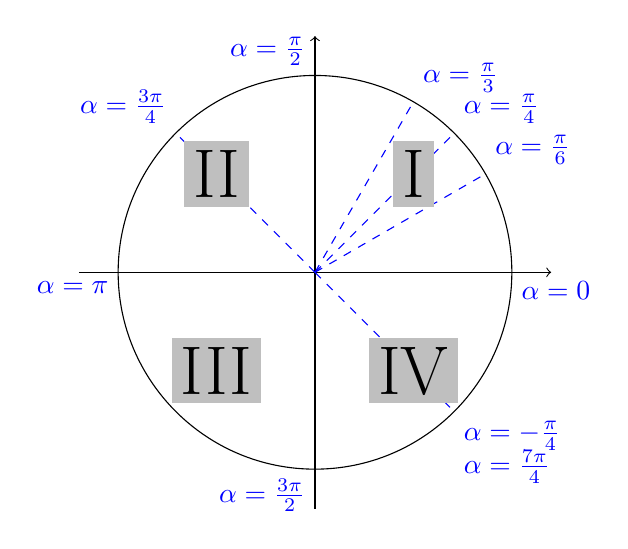
\begin{tikzpicture}[scale=2.5,baseline=(current bounding box.center)]%,cap=round,transform canvas={scale=0.5}]
	
	\tikzmath{\hoek = 20; \myc = cos(\hoek); \mys = sin(\hoek); 
		\hoekb = 20;}
	
	% Goniometrische cirkel
	\draw (0,0) circle (1cm);
	\draw[->] (-1.2,0) -- (1.2,0);% node[right] {$x$};
	\draw[->] (0,-1.2) -- (0,1.2);% node[above] {$y$};
	%	\draw  (0, 0) node [below left]  {$(0,0)$};
	\draw  ( 1, 0) node [below right] {$\color{blue}\alpha=0$};
	\draw  ( 0, -1) node [below left]  {$\color{blue}\alpha=\frac{3\pi}{2}$};	
	\draw  ( 0, 1) node [above left]  {$\color{blue}\alpha=\frac{\pi}{2}$};		
	\draw  ( -1,0) node [below left]  {$\color{blue}\alpha=\pi$};
	\draw[blue,dashed]  (0,0) -- (30:1) node [above right]  {$\color{blue}\alpha=\frac{\pi}{6}$};
	\draw[blue,dashed]  (0,0) -- (45:1) node [above right]  {$\color{blue}\alpha=\frac{\pi}{4}$};
	\draw[blue,dashed]  (0,0) -- (-45:1) node [below right,align=left]  {$\color{blue}\alpha=-\frac{\pi}{4}$\\$\alpha=\frac{7\pi}{4}$};
	\draw[blue,dashed]  (0,0) -- (60:1) node [above right]  {$\color{blue}\alpha=\frac{\pi}{3}$};
	\draw[blue,dashed]  (0,0) -- (135:1) node [above left]  {$\color{blue}\alpha=\frac{3\pi}{4}$};		
	%
	
	\draw[black]  ( 0.5, 0.5) node[fill=lightgray] {\Huge I};	
	\draw[black]  (-0.5, 0.5) node[fill=lightgray] {\Huge II};	
	\draw[black]  (-0.5,-0.5) node[fill=lightgray] {\Huge III};	
	\draw[black]  ( 0.5,-0.5) node[fill=lightgray] {\Huge IV};	
	
	\end{tikzpicture}
  
  
 % rechthoekige driehoek, met tangens en cotangens
\begin{tikzpicture}[scale=2.5,baseline=(current bounding box.center)]%,cap=round,transform canvas={scale=0.5}]
 
\tikzmath{\hoek = 35; \myc = cos(\hoek); \mys = sin(\hoek);
    \hoekb = 20;}
% Goniometrische cirkel
\draw (0,0) circle (1cm);
\draw[->] (-1.2,0) -- (1.2,0);% node[right] {$x$};
\draw[->] (0,-1.2) -- (0,1.2);% node[above] {$y$};
%   \draw  (0, 0) node [below left]  {$(0,0)$};
\draw  ( 1, 0) node [below right] {$ 1$};
\draw  (-1, 0) node [below left]  {$-1$};  
\draw  ( 0, 1) node [above left]  {$ 1$};      
\draw  ( 0,-1) node [below left]  {$-1$};
 
\draw  ( 1,-1) -- (1,1.2);  %node [right]  {$\tan\alpha$};
%\draw  ( -1,1)  node [above]  {$\cot\alpha$} -- (1.5,1) ;


%% =>>> volgende regel is horizontaal voor cot weg
%\draw  ( -1,1)  -- (1.5,1) ;
 
 
\draw (0:0)  -- (\hoek:1.4);
%\draw[color=blue,ultra thick] ({cos(\hoek)},0) -- (0:0)  -- (\hoek:1);
 
\draw[color=blue, ->] (0.3,0) arc (0:\hoek:0.3cm) node [midway,right] {$\alpha$};  
 
\draw[color=black] (\hoek:1) node[name=P,circle, fill=black, radius=1pt,scale=0.8] {} node [yshift=4pt,left] {$(x,y)$} ; 
 
\draw[blue, ultra thick] (0,0) -- ({cos(\hoek)},0);
\draw[blue, ultra thick] ({cos(\hoek)},0) node[circle, fill=black, radius=1pt,scale=0.5] {} node[below] {\color{black}$x$} -- (P);
\draw[dashed] (0,{sin(\hoek)}) node[circle, fill=black, radius=1pt,scale=0.5] {} node[left] {$y$} -- (P);
 
\draw [thick, blue,decorate,decoration={brace,amplitude=10pt,mirror},yshift=-5pt](0,0) -- ({cos(\hoek)},0) node[black,midway,yshift=-0.6cm] {\footnotesize $\cos\alpha$};
 
\draw [thick, blue,decorate,decoration={brace,amplitude=10pt},xshift=-4pt](0,0) -- (0,{sin(\hoek)}) node[black,midway,right,xshift=-1.1cm] {\footnotesize $\sin\alpha$};
 
\draw [very thick, red] (1,0) -- (1,{tan(\hoek)}) node[circle, fill=black, radius=1pt,scale=0.5] {};
\draw [thick, red,decorate,decoration={brace,amplitude=10pt,mirror},xshift=2pt](1,0) -- (1,{tan(\hoek)}) node[black,midway,right,xshift=8pt] {\footnotesize $\tan\alpha$};
 
%\draw [very thick, red] (0,1) --  ({cot(\hoek)},1) node[circle, fill=black, radius=1pt,scale=0.5] {};
%\draw [thick, red,decorate,decoration={brace,amplitude=10pt},yshift=2pt](0,1) -- ({cot(\hoek)},1) node[black,midway,above,yshift=8pt] {\footnotesize $\cot\alpha$};
 
 
\end{tikzpicture}
\end{image}

\begin{tabular}{ll}
De \textbf{cosinus} en \textbf{sinus} van $\alpha$ zijn per definitie de coördinaten van  $P_\alpha$:&
\important{P_\alpha = (\cos\alpha,\sin\alpha)} \\
De \textbf{tangens} van $\alpha$ is de verhouding van sinus tot cosinus: &
\important{\tan\alpha = \frac{\sin \alpha}{\cos \alpha}}.
\end{tabular}
% wat meetkundig tevens overeenkomt met het lijnsegment dat raakt aan de cirkel (zie figuur). \\ 

Voor scherpe hoeken volgt dan uit de stelling van Pythagoras:
% de meer gekende formules in een rechthoekige driehoek:
\newcommand{\Loverstaandezijde}{\nlentext{Overstaande zijde}{opposite side}}
\newcommand{\Laanliggendezijde}{\nlentext{Aanliggende zijde}{adjacent side}}
\newcommand{\Lschuinezijde}{\nlentext{Schuine zijde}{hypotenuse}}
$$
\begin{array}{rccl}
	 \important{\sin\alpha = \dfrac{a}{c}}  = \dfrac{\Loverstaandezijde}{\Lschuinezijde}      & \nlentext{SOS}{SOH} && \important{a = \sin\alpha \cdot c} \\
	 \important{\cos\alpha = \dfrac{b}{c}}  = \dfrac{\Laanliggendezijde}{\Lschuinezijde}      & \nlentext{CAS}{CAH} && \important{b = \cos\alpha \cdot c} \\
	 \important{\tan\alpha = \dfrac{a}{b}}  = \dfrac{\Loverstaandezijde}{\Laanliggendezijde}  & \text{TOA}          && \important{a = \tan\alpha \cdot b} \\
	% \important{\cot\alpha = \dfrac{b}{a} } & = \dfrac{1}{\tan\alpha} = \dfrac{\cos\alpha}{\sin\alpha} && b = \cot\alpha \cdot a & \Lcotangens 
\end{array}
$$

\textbf{Hoofdformule van de goniometrie}:
$\important{\cos^2\alpha + \sin^2 \alpha = 1}$.

}

\posterbox[adjusted title={Het reële vlak, met vectoren en afstand}]{
	name=r2,column=7,span=6,below=r1
}{

\begin{tikzpicture}[line cap=round,line join=round,>=triangle 45,x=0.7cm,y=0.7cm]
    \draw[->,thick] (-0.5,0) -- (8,0)node[below left]{$x$};
    \draw[->,thick] (0,-0.5) -- (0,5)node[below left]{$y$};
    \draw[thick,blue,fill=black] (2.5,4)  circle(2pt) node[above]{$Q$}
                         -- (2.5,1.5)circle(2pt) node[below left]{$R$} node(Y)[midway,left ]{$|y_2-y_1|$}
                         -- (6.5,1.5)circle(2pt) node[right]{$P$}      node(X)[midway,below]{$|x_2-x_1|$}
                         -- (2.5,4);
    \draw[line width=1pt,dash pattern=on 4pt off 3pt] (2.5,0) node[below]{$x_2$}|-(0,1.5)node[left]{$y_1$};
    \draw[line width=1pt,dash pattern=on 4pt off 3pt] (6.5,0) node[below]{$x_1$}--(6.5,1.5);
    \draw[line width=1pt,dash pattern=on 4pt off 3pt] (2.5,4)--(0,4)node[left]{$y_2$};
    \draw (2.7,1.9)|-(2.9,1.7);
    \draw[->] (Y)--(Y|-2.5,4);
    \draw[->] (Y)--(Y|-2.5,1.5);
    \draw[->] (X)--(X-|6.5,1.5);
    \draw[->] (X)--(X-|2.5,1.5);
    \draw (6,2.5) node[right] {\Large
$\small
\begin{array}{rl}
|PQ|^2 & = |PR|^2 + |RQ|^2 \\
       & = |x_2 - x_1|^2 + |y_2 - y_1|^2 \\
       & = (x_2 - x_1)^2 + (y_2 - y_1)^2
\end{array}    
$
};
\end{tikzpicture}

% \end{minipage}

De \textbf{afstand} tussen $P(x_1,y_1)$ en $Q(x_2,y_2)$ is
$ 
d(P,Q) \perdef |PQ| \perdef \important{\sqrt{ (x_2-x_1)^2 + (y_2 - y_1)^2}}
$.

}
\posterbox[adjusted title={Poolcoördinaten}]{
	name=l3,column=1,span=6,below=l2
}{

$P(a,b)$ heeft als poolcoördinaten $r=\sqrt{a2 ^+b^2}$ en $\theta=$ de hoek naar $(a,b)$.

}



\end{tcbposter}


% \begin{tcbposter}
% 	\xmpostertitle{Complexe getallen: bewerkingen}{span=4}
	
	
% 	\posterbox[adjusted title=Optellen / som]{
% 		name=l1,column=1,span=4,below=title
% 	}{
	
% 	%\textbf{Optellen / Som} 
	
% 	\begin{tikzpicture}[scale=1.5]
		
% 		\draw[thin,->] (-0.2,0)  -- (3.5,0) node[above] {$Re$};
% 		\draw[thin,->] (0,-0.2)  -- (0,2.3) node[right] {$Im$};
		
% 		\draw[blue,ultra thick, ->] (0,0) --  (3,2  ) coordinate (z1) node[above left]{$z_1=a+bi$};	
% 		\draw[blue,ultra thick, ->] (0,0) --  (2,0.5) coordinate (z2) node[below right]{$z_2=c+di$};	
		
% 		% \draw[color=red,ultra thick, ->] (0,0) -- (3,2);
% 		\draw[color=red,ultra thick, ->] (0,0) -- ($(z1)+(z2)$) node[above]{$z_1+z_2$};
% 		\draw[color=red] (0,3) node[right]{\important{z_1+z_2=(a+c)+(b+d)i}};
% 		\draw[dashed] (z2) -- ($(z1)+(z2)$) ;
% 		\draw[dashed,ultra thick, color=blue,->] (z1) -- ($(z1)+(z2)$);	
% 		%\draw (3,1.6) node[right] {\textbf{som}};	
		
% 	\end{tikzpicture}
	
% 	\begin{tabular}{ll}
% 	\textbf{Slagzin}: & Som van de reële delen, \\
% 	                  & som van de imaginaire delen.\\
% 	\textbf{Grafisch}:& Pijlen na elkaar zetten. \\
% 	\textbf{Polair}:  & Omzetten naar cartesiaans.
% 	%% \textbf{Polair}:& $re^{i\alpha}+se^{i\beta} = ???$ (geen eenvoudige formule).

% 	\end{tabular}
	
% 	}
% 	\posterbox[adjusted title=Aftrekken / verschil]{
% 		name=l2,column=1,span=4,below=l1    % could be r1, but must be replaced !
% 	}{
		
% 	%\textbf{Aftrekken}
	
	
% 	\begin{tikzpicture}[scale=1.5]
		
% 		\draw[thin,->] (-0.2,0)  -- (3.5,0) node[above] {$Re$};
% 		\draw[thin,->] (0,-0.2)  -- (0,2.3) node[right] {$Im$};
		
% 		\draw[blue,ultra thick, ->] (0,0) -- (3,2  ) coordinate (z1) node[right]{$z_1=a+bi$};
% 		\draw[blue,ultra thick, ->] (0,0) -- (2,0.5) coordinate (z2) node[below right]{$z_2=c+di$};

% %		\draw[dashed] (1,1.5) -- (3,2) ;
% 		\draw[color=red,ultra thick, ->] (0,0) -- ($(z1)-(z2)$) node[above] {$z_1-z_2$};
% 		\draw[dashed, color=blue,ultra thick, ->] (z1) -- node[above left] {$-z_2$} ($(z1)-(z2)$);
% 		\draw[color=red] (0,3) node[right]{\important{z_1-z_2=(a-c)+(b-d)i}};
% 		%\draw[color=red,ultra thick, ->] (2,0.5) -- ($(z1)-(z2)$);	
% 		%\draw[color=teal,ultra thick, ->] (0,0) -- (1,1.5);	
% 		%\draw (2.7,1) node[right] {\textbf{verschil}};	
		
% 		% \draw[color=blue,<-] (1,1.5) -- (3,2) ;
% %		
% 		\draw[color=teal,thin,dashed,->] (z2)  -- ($(z2)+(1.5,0)$) node[above] {$Re$};
% 		\draw[color=teal,thin,dashed,->] (z2)  -- ($(z2)+(0,1.9)$) node[right] {$Im$};
% 		\draw[color=red,thick,dashed,->] (z2)  -- (z1) node[right] {};
		
		
% 	\end{tikzpicture}
	
% 	\begin{tabular}{ll}
% 		\textbf{Slagzin}: & Verschil van de reële delen, \\
% 						  & verschil van de imaginaire delen.\\
% 		\textbf{Grafisch}:& Eindpunten met mekaar verbinden. \\
% 		\textbf{Polair}:  & Omzetten naar cartesiaans.
% 	\end{tabular}
	
% }
	
% \posterbox[adjusted title=Vermenigvuldigen / product]{
% 	name=r1,column=5,span=4,below=title
% }{	
	
	
% %	\begin{minipage}[t]{12cm}
% %		$(a+bi)(c+di)=(ac-bd)+(ad+bc)i$\\
% %		$ r(\cos\alpha+i\sin\alpha) \cdot s(\cos  \beta+i\sin\beta)=rs(\cos(\alpha+\beta)+i\sin(\alpha+\beta))
% %		$\\
% %		$
% %		re^{i\alpha}se^{i\beta}=rse^{i(\alpha+\beta)}
% %		$
% %	\end{minipage}

	
		
% 	\begin{tikzpicture}[scale=1.5]%,cap=round,transform canvas={scale=0.5}]
		
% 		\draw[thin,->] (-0.2,0)  -- (2.5,0) node[above] {$Re$};
% 		\draw[thin,->] (0,-0.2)  -- (0,2.2) node[right] {$Im$};
		
		
% 		\draw[blue,ultra thick, ->] (0,0) -- (1,0.3)node[right] {$z_1=re^{i \alpha}$}; 
% 		\draw[blue,ultra thick, ->] (0,0) -- (2,1.5)node[right] {$z_2=se^{i \beta}$}; 
% 		\draw[color=red, ultra thick, ->] (0,0) -- node[left] {$rs$} (1.7,2.1) node[right] {$z_1z_2$};
% 		\draw[color=red] (5,2.3) node[left] {\important{z_1z_2=rse^{i (\alpha+\beta)}}}; 	
% 		% \draw (1.7,1.7) node[right] {\textbf{produkt}};
		
% 		\draw[->] (0.6,0) arc (0:atan(0.3):0.6) node [midway,right] {$\alpha$}; 
% 		\draw[color=teal,->] (0.766,0.230) arc (atan(0.3):atan(2.1/1.7):0.76) node [midway,right] {$\beta$}; 		
% 	\end{tikzpicture}
	
% 	\begin{tabular}{ll}
% 		\textbf{Slagzin}: & Product van de moduli, \\
% 						  & som van de argumenten.\\
% 		\textbf{Grafisch}:& modulus=schaalfactor, \\ 
% 		                  & argument=rotatiehoek (fasedraaiing) \\
% 		\textbf{Cartesiaans}: & \important{(a+bi)(c+di)=(ac-bd)+(ad+bc)i}  \\
% 		                      & dus: uitwerken met $i^2=-1$
% 	\end{tabular}

	
	
% %	\hspace{1cm}\textbf{polair/exponentieel}
	
% }

% \posterbox[adjusted title=Delen / quotiënt]{
% 	name=r2,column=5,span=4,below=r1
% }{	

% %	\begin{minipage}[t]{12cm}
% %		$\displaystyle{
% %			\frac{a+bi}{c+di}=\frac{(a+bi)(c-di)}{(c+di)(c-di)}=\frac{ac+bd}{c^2+d^2}+\frac{bc-ad}{c^2+d^2}i
% %		}$\\
% %		$\displaystyle{
% %			\frac{r(\cos(\alpha)+\sin(\alpha)i)}{s(\cos(\beta)+\sin(\beta)i)}=\frac{r}{s}(\cos(\alpha-\beta)+\sin(\alpha-\beta)i)
% %		}$\\
% %		$\displaystyle{
% %			\frac{r e^{i\alpha}}{s e^{i\beta}} = \frac{r}{s} e^{i(\alpha - \beta)}
% %		}$
% %	\end{minipage}


% 	\begin{tikzpicture}[scale=1.5]%,cap=round,transform canvas={scale=0.5}]
	
% 	\draw[color=red,ultra thick, ->] (0,0) -- (1,0.3) node[right] {$\dfrac{z}{z_2}$};
% 	\draw[red]  (5,2.3) node[left] {\important{\frac{z_1}{z_2}=\frac{r}{s}e^{i (\alpha-\beta)}}}; 
% 	\draw[blue,ultra thick, ->] (0,0) -- (2,1.5) node[right] {$z_2=se^{i \beta}$}; 
% 	\draw[blue,ultra thick, ->] (0,0) -- (1.7,2.1) node[right] {$z_1=re^{i \alpha}$};

% %	\draw (1.7,1.7) node[right] ;
% %	
% 	\draw[->] (0.4,0) arc (0:atan(2.1/1.7):0.4) node [midway,right] {$\alpha$}; 
% 	\draw[color=teal,<-] (0.766,0.230) arc (atan(0.3):atan(2.1/1.7):0.76) node [midway,right] {$-\beta$}; 	

% 	\draw[thin,->] (-0.2,0)  -- (2.5,0) node[below] {$Re$};
% 	\draw[thin,->] (0,-0.2)  -- (0,2.5) node[right] {$Im$};	
% 	\end{tikzpicture}

% 	\begin{tabular}{@{}l@{}l@{}}
% 		\textbf{Slagzin}: & Quotiënt van de moduli, \\
% 						  & verschil van de argumenten.\\
% 		\textbf{Grafisch}:& modulus=schaalfactor, \\ 
% 		                  & argument=rotatiehoek (fasedraaiing) \\
% 		\textbf{Cartesiaans}: & \important{\frac{a+bi}{c+di}=\dfrac{(a+bi)\blue{(c-di)}}{(c+di)\blue{(c-di)}}=\dfrac{ac+bd}{c^2+d^2}+\frac{bc-ad}{c^2+d^2}i} \\
% 		                      & dus: teller en noemer maal \\
% 							  & complex toegevoegde van noemer.
% 	\end{tabular}

% % \hspace{1cm}\textbf{polair/exponentieel}
% }


% \posterbox[adjusted title=Machten]{
% 		name=x1,column=9,span=4,below=title
% }{	
	

% %	\begin{minipage}[t]{12cm}
% %	$r(\cos(\theta)+\sin(\theta)i)^n=r^n(\cos(n\theta)+\sin(n\theta)i)$
% %	
% %	$(re^{i\theta})^n=r^n e^{in\theta}$
% %	\end{minipage}
	
% 	\begin{tikzpicture}[scale=1.5]%,cap=round,transform canvas={scale=0.5}]
	

% 	\draw [blue, ->, ultra thick,rotate=10] (0,0) --(1.3,0) node [right] {$z=re^{i\theta}$};
	
% 	\foreach \i in {2,3,...,6} 
% 		\draw [->, ultra thick,color=red,rotate=\i*10] (0,0) -- node [color=teal, above, rotate=\i*10,pos=0.9] {\small $r^{\i}$} (1.3^\i,0) node [right, black] {$z^{\i} = r^{\i}e^{i\i\theta}$};

% 		% \draw [->, ultra thick,color=teal,rotate=20] (0,0) --(1.69,0) node [right] {$z^2$};
% 		% \draw [->, ultra thick,color=teal,rotate=30] (0,0) --(2.197,0) node [right] {$z^3$};
% 		% \draw [->, ultra thick,color=teal,rotate=40] (0,0) --(2.856,0) node [right] {$z^4$};
% 		% \draw [->, ultra thick,color=teal,rotate=50] (0,0) --(3.713,0) node [right] {$z^5$};
% 		% \draw [->, ultra thick,color=teal,rotate=60] (0,0) --(4.827,0) node [right] {$z^6$};
% 	\draw[thin,->] (-0.2,0)  -- (2.5,0) node[below] {$Re$};
% 	\draw[thin,->] (0,-0.2)  -- (0,3) node[right] {$Im$};	
	
% 	\draw[red] (0,4.5) node[right] {\important{z^n=(re^{i\theta})^n=r^n e^{in\theta}}};
% \end{tikzpicture}


% \begin{tabular}{ll}
% 	\textbf{Slagzin}: & Modulus tot de \(n\)-de macht, \\ 
% 					  & argument maal \(n\) \\
% 	\textbf{Grafisch}:& modulus=schaalfactor, \\ 
% 					  & argument=rotatiehoek (fasedraaiing) \\
% 	\textbf{Cartesiaans}:& uitwerken (Binomium van Newton) \\ 
% 	                     & of omzetten naar polair \\ 
% \end{tabular}
% }

% \posterbox[adjusted title=Wortels]{
% 		name=x2,column=9,span=4,below=x1
% }{	

% 		$z=re^{i\theta}$ heeft precies $n$ n-demachtswortels:\\
% 		 $x_k = \sqrt[n]{r}e^{i\frac{\theta + k 2 \pi}{n}}$,  met $k=0,1,\ldots,n-1$

% % \url{https://www.geogebra.org/m/By0RL6MI}

% \centering

% \scalebox{1}{
% 	\begin{tikzpicture}[scale=1.5,baseline=(current bounding box.center)]
	
% 	\tikzmath{\hoek = 20; \myc = cos(\hoek); \mys = sin(\hoek); 
% 		\hoekb = 20;}
	
	
% 	% Goniometrische cirkel
% 	\draw (0,0) circle (1cm);
% 	\draw[gray,->] (-1.2,0) -- (1.2,0);% node[right] {$x$};
% 	\draw[gray,->] (0,-1.2) -- (0,1.2);% node[above] {$y$};
% 	%	\draw  (0, 0) node [below left]  {$(0,0)$};
% 	\draw  (0,0) -- ( 0:1 ) node [align=right,above right] {$\blue{e^{0}} = 1$};
% 	\draw  (0,0) -- ( 72:1 ) node [align=right,above right] {$\blue{e^{i2\pi/5}}$};
% 	\draw  (0,0) -- ( 144:1 ) node [align=right,above left] {$\blue{e^{i4\pi/5}}$};
% 	\draw  (0,0) -- ( -144:1 ) node [align=right,below left] {$\blue{e^{i6\pi/5}}$};
% 	\draw  (0,0) -- ( -72:1 ) node [align=right,below right] {$\blue{e^{i8\pi/5}}$};
% 	\node at (0:1) [circle, fill=black, scale=0.6]{};  
% 	\node at (72:1) [circle, fill=black, scale=0.6]{};  
% 	\node at (144:1) [circle, fill=black, scale=0.6]{};  
% 	\node at (-144:1) [circle, fill=black, scale=0.6]{};  
% 	\node at (-72:1) [circle, fill=black, scale=0.6]{};  
% 	\end{tikzpicture}
% }

% Er zijn vijf 5-de wortels van $1$, namelijk $\important{e^{i2k\pi/5}}, k=0,1,2,3,4$.
% }

% \end{tcbposter}

\end{document}
